% Template for Elsevier CRC journal article
% version 1.2 dated 09 May 2011

% This file (c) 2009-2011 Elsevier Ltd.  Modifications may be freely made,
% provided the edited file is saved under a different name

% This file contains modifications for Transportation Research Procedia

% Changes since version 1.1
% - added "procedia" option compliant with ecrc.sty version 1.2a
%   (makes the layout approximately the same as the Word CRC template)
% - added example for generating copyright line in abstract

%-----------------------------------------------------------------------------------

%% This template uses the elsarticle.cls document class and the extension package ecrc.sty
%% For full documentation on usage of elsarticle.cls, consult the documentation "elsdoc.pdf"
%% Further resources available at http://www.elsevier.com/latex

%-----------------------------------------------------------------------------------

%%%%%%%%%%%%%%%%%%%%%%%%%%%%%%%%%%%%%%%%%%%%%%%%%%%%%%%%%%%%%%
%%%%%%%%%%%%%%%%%%%%%%%%%%%%%%%%%%%%%%%%%%%%%%%%%%%%%%%%%%%%%%
%%                                                          %%
%% Important note on usage                                  %%
%% -----------------------                                  %%
%% This file should normally be compiled with PDFLaTeX      %%
%% Using standard LaTeX should work but may produce clashes %%
%%                                                          %%
%%%%%%%%%%%%%%%%%%%%%%%%%%%%%%%%%%%%%%%%%%%%%%%%%%%%%%%%%%%%%%
%%%%%%%%%%%%%%%%%%%%%%%%%%%%%%%%%%%%%%%%%%%%%%%%%%%%%%%%%%%%%%

%% The '3p' and 'times' class options of elsarticle are used for Elsevier CRC
%% The 'procedia' option causes ecrc to approximate to the Word template
\documentclass[3p,times,procedia]{elsarticle}
\flushbottom

%% The `ecrc' package must be called to make the CRC functionality available
\usepackage{ecrc}
%\usepackage{amsmath}
\usepackage{multirow}
\usepackage{tabularx} % 放到导言区
\usepackage{booktabs} 

%% The ecrc package defines commands needed for running heads and logos.
%% For running heads, you can set the journal name, the volume, the starting page and the authors

%% set the volume if you know. Otherwise `00'
\volume{00}

%% set the starting page if not 1
\firstpage{1}

% %% Give the name of the journal
% \journalname{Transportation Research Procedia}

% %% Give the author list to appear in the running head
% %% Example \runauth{C.V. Radhakrishnan et al.}
% \runauth{Author name}

%% The choice of journal logo is determined by the \jid and \jnltitlelogo commands.
%% A user-supplied logo with the name <\jid>logo.pdf will be inserted if present.
%% e.g. if \jid{yspmi} the system will look for a file yspmilogo.pdf
%% Otherwise the content of \jnltitlelogo will be set between horizontal lines as a default logo

%% Give the abbreviation of the Journal.
\jid{trpro}

%% Give a short journal name for the dummy logo (if needed)
%\jnltitlelogo{Transportation Research}

%% Hereafter the template follows `elsarticle'.
%% For more details see the existing template files elsarticle-template-harv.tex and elsarticle-template-num.tex.

%% Elsevier CRC generally uses a numbered reference style
%% For this, the conventions of elsarticle-template-num.tex should be followed (included below)
%% If using BibTeX, use the style file elsarticle-num.bst

%% End of ecrc-specific commands
%%%%%%%%%%%%%%%%%%%%%%%%%%%%%%%%%%%%%%%%%%%%%%%%%%%%%%%%%%%%%%%%%%%%%%%%%%

%% The amssymb package provides various useful mathematical symbols
\usepackage{calrsfs} % For pazocal
\DeclareMathAlphabet{\pazocal}{OMS}{zplm}{m}{n}

\usepackage{amsmath} 
\usepackage{amssymb}
%% The amsthm package provides extended theorem environments
%% \usepackage{amsthm}

%% The lineno packages adds line numbers. Start line numbering with
%% \begin{linenumbers}, end it with \end{linenumbers}. Or switch it on
%% for the whole article with \linenumbers after \end{frontmatter}.
%% \usepackage{lineno}

%% natbib.sty is loaded by default. However, natbib options can be
%% provided with \biboptions{...} command. Following options are
%% valid:

%%   round  -  round parentheses are used (default)
%%   square -  square brackets are used   [option]
%%   curly  -  curly braces are used      {option}
%%   angle  -  angle brackets are used    <option>
%%   semicolon  -  multiple citations separated by semi-colon
%%   colon  - same as semicolon, an earlier confusion
%%   comma  -  separated by comma
%%   numbers-  selects numerical citations
%%   super  -  numerical citations as superscripts
%%   sort   -  sorts multiple citations according to order in ref. list
%%   sort&compress   -  like sort, but also compresses numerical citations
%%   compress - compresses without sorting
%%
\biboptions{authoryear}

% \biboptions{}

% if you have landscape tables
\usepackage[figuresright]{rotating}
%\usepackage{harvard}
% put your own definitions here:x
%   \newcommand{\cZ}{\cal{Z}}
%   \newtheorem{def}{Definition}[section]
%   ...

% add words to TeX's hyphenation exception list
%\hyphenation{author another created financial paper re-commend-ed Post-Script}

% declarations for front matter

\usepackage{xurl}
\usepackage[bookmarks=false]{hyperref}
    \hypersetup{colorlinks,
      linkcolor=blue,
      citecolor=blue,
      urlcolor=blue}


\begin{document}
\begin{frontmatter}

%% Title, authors and addresses

%% use the tnoteref command within \title for footnotes;
%% use the tnotetext command for the associated footnote;
%% use the fnref command within \author or \address for footnotes;
%% use the fntext command for the associated footnote;
%% use the corref command within \author for corresponding author footnotes;
%% use the cortext command for the associated footnote;
%% use the ead command for the email address,
%% and the form \ead[url] for the home page:
%%
%% \title{Title\tnoteref{label1}}
%% \tnotetext[label1]{}
%% \author{Name\corref{cor1}\fnref{label2}}
%% \ead{email address}
%% \ead[url]{home page}
%% \fntext[label2]{}
%% \cortext[cor1]{}
%% \address{Address\fnref{label3}}
%% \fntext[label3]{}

\dochead{World Conference on Transport Research - WCTR 2026 Toulouse 6-10 July 2026}%

\title{Proactive–Adaptive Public Transport Planning: Bus Network Redesign for Urban Rail Disruptions}

%% use optional labels to link authors explicitly to addresses:
%% \author[label1,label2]{<author name>}
%% \address[label1]{<address>}
%% \address[label2]{<address>}

\author[a]{Zihao GUO\corref{cor1}} 
\author[a]{Andrea ARALDO}
\author[a]{Mounîm A. El Yacoubi}

\address[a]{SAMOVAR, T\'el\'ecom SudParis, Institut Polytechnique de Paris, 91120 Palaiseau, France}

\begin{abstract}
%% Text of abstract
Accessibility, understood as the extent to which opportunities can be reached within a specified travel-time threshold, constitutes a central benefit of public transport systems. Although Urban Rail Transit (URT) plays a pivotal role in ensuring such accessibility, its inherent susceptibility to disruptions disproportionately affects suburban regions where alternative travel options are scarce. Existing disruption management strategies, however, often fall short: rigid proactive measures offer limited operational flexibility, whereas purely reactive responses are typically inefficient in restoring accessibility once disruptions occur. 
%
To address these limitations, this paper introduces a novel two-stage stochastic optimization framework that couples proactive infrastructure investment with adaptive operational adjustments. The first stage identifies flexible network enhancements to be implemented in advance, while the second stage optimizes bus operations dynamically in response to disruption scenarios, thereby enhancing the resilience of the overall transport system. 
%
Empirical results from a stylized case study reveal that, relative to conventional replacement strategies, the proposed framework consistently achieves higher accessibility restoration across diverse disruption scenarios. Notably, the approach not only secures substantial accessibility gains and preserves access to opportunities but also maintains at least 66.7\% path similarity with original bus routes, ensuring operational feasibility and practical implementability. 
\end{abstract}

\begin{keyword}
Proactive-Adaptive Strategy; Accessibility; Public Transport Resilience; Disruption Management; Two-Stage Stochastic Programming;  


%% keywords here, in the form: keyword \sep keyword

%% PACS codes here, in the form: \PACS code \sep code

%% MSC codes here, in the form: \MSC code \sep code
%% or \MSC[2008] code \sep code (2000 is the default)

\end{keyword}
\cortext[cor1]{Corresponding author.}
\end{frontmatter}

\email{zihao-eric.guo@ip-paris.fr}

%%
%% Start line numbering here if you want
%%
% \linenumbers

%% main text
\vspace*{-12pt}
% =============================================
% 1. Introduction
% =============================================
\section{Introduction}

Urban Rail Transit (URT) systems form the backbone of metropolitan mobility, providing high-capacity, reliable services that reduce road congestion and environmental impacts under normal operations~\citep{tan2020evacuating}. Yet this critical infrastructure remains vulnerable to diverse disruptions, from unexpected incidents to planned maintenance. Recent examples illustrate this persistent fragility: a fire at New York City's 145th Street Station suspended service for over two hours during morning peak~\citep{barone2017abcdfire}, while recurring closures on Paris's RER B line have severely affected nearly 200,000 daily passengers despite replacement bus deployments~\citep{actu2024travaux}. Even highly reliable systems like Hong Kong's Mass Transit Railway experience hundreds of annual disruptions~\citep{zhang2020metro}. These cases reveal a fundamental challenge—conventional disruption management often fails to address passengers' actual mobility needs.

The fallout from urban rail transit (URT) disruptions signifies more than mere delays; it represents a critical failure of access. This is especially true for transit-reliant populations making essential trips. Although city centers may have redundant routes, suburbs with thinner networks are far more vulnerable; a single disruption there can completely cut people off from vital destinations such as jobs, schools, or hospitals~\citep{liu2024measuring}. Consequently, traditional metrics like average delay provide an incomplete picture by focusing solely on operational efficiency. A more comprehensive and critical metric is \emph{accessibility}, defined as the practical ability to reach important daily destinations within a reasonable time frame~\citep{miller2020measuring}. As such, maintaining accessibility during disruptions is a cornerstone of urban equity, economic inclusion, and overall resilience.

Yet, current disruption management tools aren’t well-equipped to protect that kind of access. The go-to solution—substitute buses along the affected rail corridors—tends to recreate the form of service without delivering the function. People may technically have a way to travel, but whether they can still reach their destinations efficiently is another question~\citep{ieda1995commuter}. This points to a deeper disconnect: recovering service is not the same as restoring mobility. While research has made strides on both proactive infrastructure planning (say, adding redundant lines) and reactive operational fixes (like shifting train schedules), the two strategies rarely intersect. The former can be rigid and costly; the latter, often ad hoc and narrowly focused, typically overlooks broader accessibility impacts.

To address this gap, we introduce a new framework for redesigning bus networks in the face of URT disruptions. Unlike traditional models, ours combines long-term planning with real-time adaptability, all while optimizing explicitly for \emph{accessibility}. The approach uses a two-stage stochastic optimization model: in the first stage, the system prepares network elements; in the second, it dynamically adjusts routes and service frequencies in response to actual disruption scenarios. Importantly, the model incorporates practical constraints like preserving route stability to reduce user disorientation.

The framework proves its effectiveness in simulations by consistently outperforming conventional replacement strategies. It delivers superior accessibility, reliably adheres to the 30-minute threshold for possible opportunities, and maintains a minimum of 66.7\% path similarity.

% =============================================
% 2. Related Work
% =============================================
\section{Related Work}

In practice, most transit operators depend on reactive measures when a disruption. The most common approach is the implementation of replacement buses, also referred to as bus bridging services, that serve the same stops of a disrupted rail line~\citep{Pender2012,CurrieMuir2017}. Other operational strategies include stop skipping~\citep{Tang2018}, short turning~\citep{Peled2021}, speed changing~\citep{Manasra2019}, and holding~\citep{Olvera2023}, with a comprehensive overview in~\citep{Gkiotsalitis2022}.
%
However, such reactive measures are generally ad-hoc and locally focused, typically designed only to provide a minimal degree of service continuity. 
Consequently, they are rarely optimized from a system-level perspective and are often of limited benefit for the users. 
For instance, \citet{CurrieMuir2017} show that replacement buses often suffer from inadequate capacity, longer travel times, and poor reliability compared to the original rail system.

% --------------------- relatedWork.2
\subsection{Proactive Infrastructure and Resilience Planning}

In this context, it is important to clarify terminology. \emph{Robustness} refers to the ability of a network to preserve its intended function under specified disturbances without major structural or operational changes, typically involving limited performance loss under predefined failures \citep{Cats2016,Ge2022,JRC2015}.
By contrast, \emph{resilience} encompasses the capacity of the system to absorb shocks, adapt to disruptions, and recover performance over time~\citep{NRC2012,TierneyBruneau2007,Bruneau2003}.

One important stream of the literature emphasizes long-term proactive planning to enhance the resilience of PT networks. 
The idea is to anticipate possible disruptions in advance and to mitigate their impacts by strengthening the network structure 
before disruptions occur. 
This includes strategies such as designing redundant routes, reinforcing critical infrastructure components, 
increasing multimodal connectivity, and incorporating route alternatives during the initial system design~\citep{Codina2014,LiWang2019,CatsJenelius2014,Jin2014}. 
Vulnerability analysis and resilience analysis are two fundamental approaches in this field of research. 
% \todoi{aa: Check the publications of Angelo Furno and Fayçal A. TOUZOUT, who will be present in your CSI. They have work related to resilience and robustness, you want to show you do not neglect their work!}
For example, vulnerability analysis aims to identify components (stations, track segments, or links) that are most susceptible to disruptions 
or whose failure would have the most severe system-wide impact~\citep{DeLosSantos2012,RodriguezNunez2014}. 
Resilience analysis, on the other hand, evaluates the ability of the system to absorb shocks, adapt to disruptions, and recover performance 
rapidly~\citep{XuChopra2022,ChenMillerHooks2012}. 
Scholars have developed a wide range of resilience metrics, including redundancy-based indices, 
mean-excess criticality probabilities, and resilience cycles, to characterize the robustness of URT systems under disruption conditions~\citep{Zhang2015topology, XuChopra2022}.
Nevertheless, these approaches are inherently static and often conservative. 
Studies such as \citet{LiWang2019} and \citet{CatsJenelius2014} primarily rely on network analysis or vulnerability indicators, 
but remain at an analytical level and lack practical preventive solutions. 
Moreover, even in highly reliable systems such as the Hong Kong MTR, hundreds of disruptions occur annually~\citep{zhang2020metro}, underscoring that static redundancy alone cannot sufficiently address the dynamic and stochastic nature of real-world disruptions~\citep{Besinovic2020,Lusby2018}.

% --------------------- relatedWork.3
\subsection{Adaptive and Reactive Operational Strategies}

Following the common distinction in the public transport planning literature, we use the term \textit{design} to refer to strategic and tactical level decisions that are typically made in advance and updated infrequently, such as network layout, timetable construction, or fleet assignment \citep{Desaulnier2007}, \citep[Section~1.5.2]{Cascetta2009}. By contrast, we use the term \textit{operations} to indicate short-term and real-time control actions carried out during daily service execution, including vehicle dispatching, timetable adjustments, and disruption management \citep[Ch.~13]{Gkiotsalitis2022}.

In parallel with proactive strategies, a large body of research has focused on adaptive and reactive operations 
that are implemented immediately after disruptions occur. 
These studies concentrate on short-term operational measures such as train rescheduling, bus bridging service design, 
short-turning operations, and dynamic timetable adjustments. 
For example, train rescheduling has been extensively studied as one of the primary measures to alleviate the effect of rail disruptions~\citep{Cacchiani2014,Xu2017,Veelenturf2016,ZhuGoverde2020}. 
Models in this field consider timetable reconfiguration, rolling stock circulation, skip-stopping patterns, and real-time rerouting 
to minimize passenger delays, operational costs, and adjustment deviations~\citep{Kang2015,Corman2012}. 
Another stream of research investigates bus bridging strategies as an emergency replacement service. 
Here, scholars have explored route design~\citep{Jin2016,vanDerHurk2016,Deng2018}, 
bus dispatching strategies~\citep{Wang2014,Yuan2025}, and the layout of depots or standby bus resources~\citep{Pender2014,Pender2015}. 
Although these approaches can substantially mitigate passenger inconvenience in the aftermath of disruptions, their reliance on ad-hoc heuristics and case-specific solutions limits their scalability and transferability. 
In practice, every new disruption often requires the development of a new set of rules or schedules, which increases response times and risks inconsistent service quality across events. 
Moreover, such fragmented methods tend to optimize local performance (e.g., one disrupted corridor) without considering system-wide implications such as vehicle and crew availability in the broader network. 
The absence of a unified framework also makes it difficult to evaluate cost-benefit trade-offs or to systematically reuse effective strategies across different disruption scenarios. 
For instance, \citet{binder2017multi} and \citet{van2018passenger} 
demonstrate that passenger-oriented rescheduling or rolling stock adjustments can improve service quality, but the solutions remain narrowly tailored to specific cases rather than contributing to a transferable and consistent decision-support system.

% --------------------- relatedWork.4
\subsection{Integrated Design and Operations Approaches}

Recognizing the limitations of purely proactive or purely reactive approaches, 
recent research has attempted to integrate design and operations into unified frameworks. 
This includes the use of stochastic and robust optimization models that explicitly account for disruption scenarios 
when designing network structures and planning operations~\citep{Cadarso2015,CadarsoMarin2014b}.
Such models aim to capture both long-term infrastructure decisions (e.g., where to invest in redundancy or capacity) 
and short-term adaptive responses (e.g., how to reschedule services or deploy bridging resources once disruptions occur). 
For instance, robust network design methods have been proposed to incorporate demand uncertainty and infrastructure vulnerability, 
thus ensuring stable performance even under adverse conditions~\citep{CadarsoMarin2014b,AnLo2016}. 
Similarly, stochastic optimization frameworks have been used to jointly consider the probability of disruptions 
and the operational responses needed for recovery~\citep{Cadarso2015}. 

Despite these advances, current studies still exhibit clear shortcomings. 
Many frameworks place a strong emphasis on preventive robustness, which often results in conservative and costly designs, 
while others concentrate on narrowly defined reactive measures that are tailored to specific disruption cases. 
For example, \citet{LopezRamos2017} jointly optimize rapid transit network design and service frequency, yet their formulation is confined to strategic planning under nominal conditions and does not incorporate disruption recovery, leaving the integration of network design and real-time operations unaddressed.
As highlighted by \citet{Besinovic2020,Lusby2018}, the essential challenge is that existing research rarely achieves true integration. 
Strategic infrastructure planning and operational disruption management are still treated separately, 
and there is a lack of holistic models that coordinate both dimensions within a unified optimization framework.

% --------------------- relatedWork.
\subsection{Research gap: implications of perturbations and remediation to accessibility}

Transportation systems are frequently subject to perturbations such as infrastructure failures, extreme weather, or unforeseen operational incidents. These disruptions can degrade system performance in ways that directly affect users’ ability to reach destinations and maintain their daily mobility.
Despite the amount and high quality of previous work on PT disruption remediation, all previous studies have overlooked the most crucial factor of a transportation system, i.e., \emph{accessibility}~\citep{hansen1959accessibility,miller2020measuring}, which can be simply defined as the ease with which people can reach desired opportunities such as jobs, services, or social activities. This aspect is particularly important in suburban regions, where accessibility often tightly depends on one or a few PT lines. Due to the scarcity of public transport alternatives, a disruption of a PT line can severely impact the accessibility of suburbs, preventing transit-reliant residents from performing their daily activities and reinforcing existing social inequities~\citep{lucas2012transport,karner2018assessing}.

While accessibility is a well-established concept in transportation planning~\citep{geurs2004accessibility,handy1997measuring,miller2020measuring}, our investigation confirms that URT disruption management research has not explicitly incorporated it as an optimization objective. The authors of~\citet{liu2024measuring} define accessibility as ``the potential of opportunities for interaction'' and recognize that transit systems face a high risk of degradation from external disruptions, affecting their ability to deliver reliable accessibility. Their work introduces measures to detect disruptions' impacts on accessibility, but focuses on measurement rather than intervention. Similarly, \citet{nalin2025evaluation} emphasizes the necessity of assessing the actual performance of public transportation rather than relying on schedules when evaluating accessibility, yet does not propose recovery strategies. 
%
This critical gap in the literature, the absence of optimization methods to restore accessibility through network redesign, constitutes our paper's core contribution.

% ------------------------ Contribution
\subsection{Our Contribution}

To the best of our knowledge, we are the first to propose a bus network redesign methodology for Urban Rail Transit (URT) disruptions that jointly integrates preventive planning and adaptive operations. 
Our framework combines strategic design of potential bus routes and resources before disruptions with adjustments after disruptions, thereby unifying robustness and resilience within a single model. 
This integration avoids the excessive conservatism and cost of purely preventive designs while overcoming the passivity and inefficiency of purely reactive responses. 
A key novelty of our work is the explicit incorporation of \emph{accessibility} as the optimization objective. 
Whereas existing disruption studies primarily rely on efficiency metrics such as travel time or cost, 
we focus on restoring passengers’ ability to reach opportunities across the network. 
This accessibility-oriented perspective not only reflects the fundamental purpose of public transport systems but also fills a critical gap in the disruption management literature.


% =============================================
% 3. Preliminaries
% =============================================
\section{Preliminaries}
In this section, we introduce the basic elements of our resilient and adaptive public transport (PT) network design problem. 
Here, \emph{resilience} refers to the ability of the system to sustain service when parts of the infrastructure are disrupted, while \emph{adaptiveness} captures the flexibility to adjust bus services in response to changing conditions. 
%
Formally, the system is defined as a 4-tuple 
$\Sigma = (\pazocal{S}, \pazocal{G}, \pazocal{L}, \Omega)$,
where $\pazocal{S}$ is the spatial tessellation of the study area, $\pazocal{G}$ the physical infrastructure graph, $\pazocal{L}$ the set of PT service lines, and $\Omega$ the set of disruption scenarios. 
%
The following subsections provide a detailed description of each component.

% --------------------------------- 3.1
\subsection{Tessellation of the Study Area}
We partition the study area into a regular tessellation of spatial tiles. Let $\pazocal{S}$ denote the set of tiles, and $c_s$ the geometric centroid of tile $s \in \pazocal{S}$. The set of centroids is $\pazocal{C} = \{c_s : s \in \pazocal{S}\}$. 
%
A traveler can either walk directly at speed $v_{walking}$ or combine walking with PT, such as walking from $c_i$ to an urban rail station or bus stop, taking PT, and then walking from the alighting point to $c_j$. Although centroid-to-centroid distances do not perfectly match actual paths, they provide a reasonable approximation for network-scale analysis.

If a tile contains existing bus stops, walking times $w_{sj}$ from its centroid $c_s$ to each stop $j$ are precomputed. 
Tiles without stops are instead assigned a candidate stop at $c_s$. 
For each tile $s$, we also define a set of accessible opportunities $\pazocal{O}_s$, 
meaning the activity locations (such as workplaces, schools, or healthcare facilities) that can be reached from $c_s$. 
Accessibility is understood as the ease of reaching such opportunities within a given travel time, 
and a detailed measure will be introduced in Section~\ref{sec:TWA}.

% --------------------------------- 3.2
\subsection{Graph Representation of the PT Network}
The PT network is represented by a multi-layer graph $\pazocal{G} = (\pazocal{N}, \pazocal{E})$ that captures both existing infrastructure and potential expansions. The node set $\pazocal{N} = \pazocal{N}^r \cup \pazocal{N}^b \cup \pazocal{N}^c$ consists of urban rail stations $\pazocal{N}^r$, existing bus stops $\pazocal{N}^b$, and candidate bus stops $\pazocal{N}^c$. The edge set $\pazocal{E} = \pazocal{E}^r \cup \pazocal{E}^b \cup \pazocal{E}^c$ includes urban rail links $\pazocal{E}^r$ connecting adjacent stations with travel times $t_{ij}^r$, existing bus connections $\pazocal{E}^b$ with travel times $t_{ij}^b$, and potential new bus links $\pazocal{E}^c$ that may connect candidate stops to existing ones or to other candidates.

% --------------------------------- 3.3
\subsection{Service Layer of the PT Network}
PT services are structured around two primary modes: urban rail and bus. %
Urban rail lines $\pazocal{L}^r$ run on fixed routes and timetables, providing the stable backbone of the network.  
Bus lines $\pazocal{L}^b$, in contrast, are more flexible. They can be adjusted when rail disruptions occur or when bus travel times become uncertain. Such adjustments may involve rerouting existing services or incorporating candidate stops, thereby ensuring continuity of coverage and sustaining overall system performance.  
%
Formally, each line $\ell \in \pazocal{L}$ is represented by a route $\pazocal{R}_\ell$, modeled as a simple path from an origin to a destination.  

% --------------------------------- 3.4
\subsection{Disruption Scenarios}
Uncertainty in the system is represented by a pair of random components, $\xi = (\xi^{\text{disruption}}, \xi^{\text{travel}})$.  
The first component, $\xi^{\text{disruption}} = \{d_{ij} : (i,j) \in \pazocal{E}^r\}$, captures rail link failures, where $d_{ij}=1$ indicates that rail edge $(i,j)$ is disrupted and therefore unavailable. %
The second component, $\xi^{\text{travel}} = \{t_{ij}^b : (i,j) \in \pazocal{E}^b \cup \pazocal{E}^c\}$, models stochastic variation in bus travel times, reflecting congestion or other operational uncertainties.  

These preliminaries provide the foundation for the resilient and adaptive PT network design problem, on which we build the formal optimization model in Section~\ref{sec:problemFormulation}.

% ---------------------------------------------------
% table
% ---------------------------------------------------
% ==================== Sets ====================
\begin{table}[h]
\caption{Sets and indices used in the model formulation.}
\begin{tabularx}{\hsize}{@{\extracolsep{\fill}}lX@{}}
\toprule
Symbol & Description \\
\colrule
$\pazocal{S}$ & Set of spatial tiles, representing the origin zones of the study area. Each element is indexed by $s$. \\

$\pazocal{O}_s$ & Set of activity opportunities (such as jobs, schools, or healthcare facilities) that are linked to a given origin tile $s \in \pazocal{S}$. Elements are indexed by $k$. \\

$\pazocal{N}$ & Set of all nodes in the public transport network. It is divided into three subsets: $\pazocal{N}^r$ (urban rail stations), $\pazocal{N}^b$ (existing bus stops), and $\pazocal{N}^c$ (candidate bus stops). Nodes are indexed by $i$ or $j$. \\

$\pazocal{E}$ & Set of all directed edges in the network, describing possible connections between nodes. It includes $\pazocal{E}^r$ (urban rail edges), $\pazocal{E}^b$ (existing bus edges), $\pazocal{E}^c$ (candidate bus edges), and $\pazocal{E}^t$ (walking transfer edges). Each edge is indexed by an ordered pair $(i,j)$ with $i,j \in \pazocal{N}$. \\

$\pazocal{L}$ & Set of all public transport service lines. This includes $\pazocal{L}^r \subseteq \pazocal{L}$ (urban rail lines) and $\pazocal{L}^b \subseteq \pazocal{L}$ (bus lines). A line $\ell \in \pazocal{L}$ is represented as an ordered sequence of stops or stations connected by edges. Lines are indexed by $\ell$. \\

$\Omega$ & Set of disruption scenarios, which represent external disturbances such as rail link failures or changes in bus travel conditions. Each scenario is indexed by $\omega$. \\
\botrule
\end{tabularx}
\end{table}

% ==================== Parameters ====================
\begin{table}[h]
\caption{Parameters used in the model formulation.}
\begin{tabularx}{\hsize}{@{\extracolsep{\fill}}lX@{}}
\toprule
Symbol & Description \\
\colrule
\multicolumn{2}{l}{\textbf{Travel-time related}} \\
$\bar{t}_{sj}^{\text{access}}$ & Walking time from an origin tile $s \in \pazocal{S}$ to an entry stop or station $j \in \pazocal{N}$ (minutes). \\
$\bar{t}_{ik}^{\text{egress}}$ & Walking time from a network node $i \in \pazocal{N}$ to an activity opportunity $k \in \pazocal{O}_s$ (minutes). \\
$\bar{t}_{ij}^{\text{transfer}}$ & Walking time required to transfer across a walking edge $(i,j) \in \pazocal{E}^t$ (minutes). \\
$\bar{t}_{ij}^r$ & In-vehicle travel time on a rail edge $(i,j) \in \pazocal{E}^r$ (minutes). \\
$\bar{w}_i^r$ & Average waiting time at rail station $i \in \pazocal{N}^r$ (minutes). \\
$\bar{t}_{ij}^\ell$ & Nominal bus travel time on edge $(i,j) \in \pazocal{E}^b \cup \pazocal{E}^c$ when operated by line $\ell \in \pazocal{L}^b$ (minutes). \\
$\bar{t}_{sk}^{\text{walk}}$ & Direct walking time between origin tile $s \in \pazocal{S}$ and opportunity $k \in \pazocal{O}_s$ (minutes). \\

\multicolumn{2}{l}{\textbf{Cost and budget}} \\
$c_i^{\text{stop}}$ & Fixed construction cost for opening a candidate stop $i \in \pazocal{N}^c$. \\
$c_{ij}^{\text{lane}}$ & Additional cost of installing a dedicated bus lane along edge $(i,j) \in \pazocal{E}^b \cup \pazocal{E}^c$. \\
$B$ & Total available investment budget for stops, lanes, and related infrastructure. \\

\multicolumn{2}{l}{\textbf{Thresholds and constants}} \\
$\tau$ & Accessibility threshold (30 minutes). \\
$\theta$ & Upper bound on expected waiting time at stops (15 minutes). \\
$\kappa$ & Constant from the random–arrival waiting time rule ($\kappa = 30$ minutes, since $\mathbb{E}[\text{wait}] = 60/(2f)$ with $f$ in veh/h). \\
$\epsilon$ & A small positive constant used to avoid boundary ambiguity in Big–$M$ constraints. \\
$M$ & A sufficiently large constant used for linearization (Big–$M$). \\

\multicolumn{2}{l}{\textbf{Scenario and model parameters}} \\
$p_\omega$ & Probability of disruption scenario $\omega \in \Omega$ 
(satisfying $\sum_{\omega \in \Omega} p_\omega = 1$). \\
$\bar{d}_{ij}^\omega$ & Disruption indicator for rail edge $(i,j) \in \pazocal{E}^r$ under scenario $\omega \in \Omega$ ($1$ if disrupted, $0$ otherwise). \\
$\mu_{\text{bus}}$ & Sensitivity factor capturing how bus travel times increase due to congestion under rail disruptions. \\
$\alpha$ & Reduction factor in bus travel times when a dedicated bus lane is installed. \\
$\lambda$ & Weight parameter balancing accessibility improvements against investment costs. \\
\botrule
\end{tabularx}
\end{table}

% ==================== Decision Variables ====================
\begin{table}[h]
\caption{Decision variables used in the model formulation.}
\begin{tabularx}{\hsize}{@{\extracolsep{\fill}}lX@{}}
\toprule
Symbol & Description \\
\colrule
\multicolumn{2}{l}{\textbf{First-stage (Design)}} \\
$z_i \in \{0,1\}$ & 1 if candidate stop $i \in \pazocal{N}^c$ is constructed; 0 otherwise. \\
$b_{ij} \in \{0,1\}$ & 1 if a dedicated bus lane is installed on edge $(i,j) \in \pazocal{E}^b \cup \pazocal{E}^c$; 0 otherwise. \\
$x_{ij}^\ell \in \{0,1\}$ & 1 if bus line $\ell \in \pazocal{L}^b$ is operated on edge $(i,j) \in \pazocal{E}^b \cup \pazocal{E}^c$; 0 otherwise. \\

\multicolumn{2}{l}{\textbf{Second-stage (Operational, per scenario $\omega \in \Omega$)}} \\
$f^{\ell,\omega} \geq 0$ & Service frequency of bus line $\ell \in \pazocal{L}^b$ under scenario $\omega$ (veh/h). \\
$y_{ij}^{sk\omega} \in \{0,1\}$ & 1 if OD pair $(s,k)$ travels on edge $(i,j) \in \pazocal{E}$ in scenario $\omega$; 0 otherwise. \\

\multicolumn{2}{l}{\textbf{Auxiliary (Structural / Linearization)}} \\
$u_{ij}^{\ell,sk\omega} \in \{0,1\}$ & 1 if OD pair $(s,k)$ uses bus line $\ell$ on edge $(i,j) \in \pazocal{E}^b \cup \pazocal{E}^c$; 0 otherwise. \\
$t_i^{\ell,sk\omega} \in \{0,1\}$ & 1 if OD pair $(s,k)$ boards bus line $\ell$ at stop $i \in \pazocal{N}^b \cup \pazocal{N}^c$; 0 otherwise. \\
$t_i^{r,sk\omega} \in \{0,1\}$ & 1 if OD pair $(s,k)$ boards urban rail at station $i \in \pazocal{N}^r$; 0 otherwise. \\
$\delta^{sk\omega} \in \{0,1\}$ & 1 if OD pair $(s,k)$ chooses public transport in scenario $\omega$; 0 if walking directly. \\
$\xi_{ij}^{\ell,sk\omega} \in \{0,1\}$ & Auxiliary variable for the product $b_{ij} \cdot u_{ij}^{\ell,sk\omega}$. \\
$\alpha_{sk\omega} \in \{0,1\}$ & 1 if OD pair $(s,k)$ is accessible in scenario $\omega$; 0 otherwise. \\
$\gamma_{sk\omega} \geq 0$ & Contribution of opportunity $k$ to the accessibility of origin $s$ in scenario $\omega$. \\

\multicolumn{2}{l}{\textbf{Derived (Definitional)}} \\
$BT_{ij}^{\ell,sk\omega}$ & Bus in-vehicle travel time on edge $(i,j) \in \pazocal{E}^b \cup \pazocal{E}^c$ (minutes). \\
$WT_{i\ell}^{sk\omega}$ & Waiting time for OD pair $(s,k)$ for line $\ell$ at stop $i \in \pazocal{N}^b \cup \pazocal{N}^c$ (minutes). \\
$T^{sk\omega}_{\text{PT}}$ & Public transport journey time of OD pair $(s,k)$ under scenario $\omega$ (minutes). \\
$T^{sk\omega}$ & Realized travel time of OD pair $(s,k)$ (minutes). \\
$A^{s,\omega}$ & Accessibility score of origin tile $s \in \pazocal{S}$ in scenario $\omega$. \\
\botrule
\end{tabularx}
\end{table}

% ---------------------------------------------------
% tableEnd
% ---------------------------------------------------

% =============================================
% 4. Methodology
% =============================================
\section{Methodology}
In this section, we develop the methodological framework for the resilient and adaptive PT network design problem. 
The objective is to restore accessibility under urban rail transit (URT) disruptions and stochastic variation in bus travel times. 
%
We proceed in two steps. 
First, we formulate the network redesign problem, where existing bus lines may be modified by rerouting or adding candidate stops in order to compensate for the loss of rail connectivity. 
Second, 
% 
...
% we construct a two-stage integer programming model that determines the optimal allocation of the bus fleet across the redesigned network, balancing operational efficiency with improved accessibility.


% --------------------------------- 4.1
\subsection{Problem Statement}
Urban rail disruptions, together with uncertainty in bus travel times, can severely compromise network accessibility. This research addresses the challenge through a strategic redesign of bus services that integrates both structural and operational aspects of the transit system. The optimization framework focuses on three main decisions:
(a) adapting the topology of bus lines during rail disruptions and uncertain road conditions, including rerouting services and adding candidate stops to maintain coverage;
(b) setting service frequencies for each line while accounting for variability in travel times; and
(c) allocating the available bus fleet efficiently across the redesigned network.

The proposed approach is designed to be practical. Transit operators increasingly rely on real-time navigation systems such as onboard consoles or tablets, which provide turn-by-turn guidance to drivers. These tools make it possible to follow revised routes during disruptions with minimal additional hardware or training, ensuring that operational changes can be implemented quickly.

As illustrated in Fig.~\ref{fig:PT_repre}, decision making under disruption takes place in two stages. In the pre-event period, operators establish an a priori preparedness plan that defines structural adjustments and allocates flexible resources. Once a disruption occurs and accurate information becomes available, the process shifts to the post-event period, where several possible scenarios may materialize. At this stage, an adaptive emergency response is required to reconfigure bus services according to the realized conditions. Disrupted rail stations are deactivated and the associated edges are removed. Let $\pazocal{D}$ denote the set of disrupted stations. Passengers at $d \in \pazocal{D}$ are directed by the central system, through phone alerts or station signage, to transfer to redesigned bus services at designated consolidation nodes. Each disrupted station can be linked either to a nearby bus stop in $\pazocal{S}$ or to the station itself, and the set of such nodes is denoted by $\pazocal{N}$.

% ------------------------- FIGframework
\begin{figure}[htbp]
\centering
\includegraphics[width=.75\textwidth]{Figure/framework.jpg}
\caption{Two-Stage Framework for Preparedness and Adaptive Response under Disruptions}\label{fig:PT_repre}
\end{figure}
% ------------------------- FIGframeworkEnd

% ----------------- 4.2.1
\subsubsection{Path Order Preservation Rate (POPR)}\label{subsec:porp}
To promote consistency between redesigned bus lines and their original service structure, we introduce the Path Order Preservation Rate (POPR). This metric quantifies the proportion of consecutive segments from an original route that are preserved in the redesigned one, thereby enhancing operational stability and reducing passenger disorientation.
%
Let the original route be represented by the node sequence $P = [v_1, v_2, \dots, v_n]$ and the redesigned route by $P' = [v'_1, v'_2, \dots, v'_m]$. Define $\pazocal{S} = \{(v_i, v_{i+1}) \mid 1 \leq i \leq n-1\}$ as the set of consecutive node pairs in $P$. A pair $(v_i, v_{i+1}) \in \pazocal{S}$ is considered preserved if $P'$ contains either the directed edge $(v_i,v_{i+1})$ or $(v_{i+1},v_i)$. Let $K$ be the number of preserved pairs and $T = |\pazocal{S}| = n-1$. The POPR is then defined as
\begin{equation}
    \text{POPR}(P,P') = \tfrac{K}{T}.
\end{equation}

This formulation is related to the \emph{path overlap ratio}, which quantifies shared link length relative to a reference path~\citep{Lim2005PathOverlap}. The POPR provides a discrete, topology-oriented counterpart by emphasizing stop sequence preservation, thereby capturing structural similarity, keeping redesigned lines close to their original topology, and mitigating passenger disorientation as well as driver operational complexity.
% ----------------- 4.2.2
\subsubsection{Accessibility}\label{sec:TWA}
Accessibility reflects how easily people can reach opportunities, such as workplaces, schools, healthcare facilities, or other essential activity locations. 
%
For each tile $s \in \pazocal{S}$, we define a set of opportunities $\pazocal{O}_s$ that are reachable from its centroid $c_s$.  
%
A classical way to measure accessibility is through gravity-based formulations~\citep{hansen1959accessibility,geurs2004accessibility},
where opportunities are weighted inversely by travel time.
In this framework, the accessibility of a centroid $c_i \in \pazocal{C}$ is expressed as
\begin{equation}
    \text{acc}(c_i, \pazocal{G}) = \sum_{c_j \in \pazocal{C}, \, c_j \neq c_i} \frac{O_{c_j}}{T_{\pazocal{G}}(c_i, c_j)},
\end{equation}
where $O_{c_j}$ is the number of opportunities in tile $c_j$, 
and $T_{\pazocal{G}}(c_i, c_j)$ is the shortest travel time between centroids $c_i$ and $c_j$ on network $\pazocal{G}$. 
This captures the intuitive idea that accessibility decreases as travel time increases.  

To better reflect practical conditions, we introduce a time-weighted variant that emphasizes opportunities reachable within 30 minutes,
a cumulative-opportunity threshold widely used in transport planning~\citep{geurs2004accessibility}.
For each tile $s \in \pazocal{S}$ under scenario $\omega \in \Omega$, we define
\begin{equation}
    A_{s,\omega} = \sum_{k \in \pazocal{O}_s} \max\left(0, \frac{30 - T_{sk}^\omega}{30}\right),
    \label{eq:Acc}
\end{equation}
where $T_{sk}^\omega$ is the travel time from centroid $c_s$ to opportunity $k$ in scenario $\omega$.  

In this formulation, an opportunity contributes a full score when it can be reached immediately, 
but its value decreases linearly with travel time and becomes zero once the 30-minute limit is exceeded. 
Compared with the gravity-based measure, this approach places greater emphasis on nearby opportunities, 
making it more sensitive to accessibility changes caused by rail disruptions and bus travel time uncertainty.

% ----------------- 4.2.3
\subsubsection{Travel Time Components}
\label{subsubsec:travel_time}

\textit{Operational background.} 
Each line $\ell$ operates with cycle time $t^\ell$ and fleet size $n^\ell$, which jointly determine the headway $h^\ell = t^\ell/n^\ell$ and the service frequency $f^\ell = 1/h^\ell$. Under the assumption of uniformly distributed passenger arrivals, the expected waiting time equals $h^\ell/2$~\citep{osuna1972control,pinto2020joint}. The time spent in the PT service between two stations, $s_j$ and $s_{j+1}$, is $t(s_j,s_{j+1})$, while the dwell time spent at a service point $s_j$, is $d_{s_j}$.

\textit{Passenger-time decomposition.}
The total journey of each passenger is represented by five components, each corresponding to a distinct phase on the public transport network: 
\textbf{access walking} $T^{sk\omega}_{\text{access}}$ (walking from the origin tile $s$ to the first entry point), 
\textbf{waiting time} $T^{sk\omega}_{\text{wait}}$ (delay at stops or urban rail stations before boarding),
\textbf{in-vehicle travel} $T^{sk\omega}_{\text{ivt}}$ (on-board time while traversing service edges, including dwell),
\textbf{transfer walking} $T^{sk\omega}_{\text{transfer}}$ (walking between services when changing lines or modes), and 
\textbf{egress walking} $T^{sk\omega}_{\text{egress}}$ (walking from the last service point to the destination opportunity $k$).
%
The \emph{PT-based journey time} of od pairs $(s,k)$ in scenario $\omega$, where $s$ represents the origin tile, $k$ signifies the destination opportunity, and $\omega$ denotes the disruption scenario, is articulated in a basic format as
\begin{equation}
T^{sk\omega}_{\text{PT}}
\;=\;
T^{sk\omega}_{\text{access}}
\;+\;
T^{sk\omega}_{\text{wait}}
\;+\;
T^{sk\omega}_{\text{ivt}}
\;+\;
T^{sk\omega}_{\text{transfer}}
\;+\;
T^{sk\omega}_{\text{egress}} .
\label{eq:tt1_general}
\end{equation}
%
For origin--destination pairs where direct walking is feasible, the traveler selects the faster alternative:
\begin{equation}
T^{sk\omega} \;=\; \min \{T^{sk\omega}_{\text{PT}}, T^{sk\omega}_{\text{walk}}\},
\label{eq:tt1_walk}
\end{equation}
where $T^{sk}_{\text{walk}}$ is the pre-computed direct walking time between tile $s$ and opportunity $k$. The specific formulations and linearizations of each component are introduced in Section~\ref{sec:problemFormulation}.

\textit{Bus time with congestion and dedicated lane effect.}
This component accounts for two effects: bus travel times rise when rail links are disrupted, with multipliers up to 2.0 observed in practice~\citep{dft2018congestion}, and dedicated bus lanes shorten travel times by about 18\% on average~\citep{russo2022buslane}. If an edge $(i,j)$ on line $\ell$ is not assigned to OD pair $(s,k)$, the travel time contribution is zero.  
%
For OD pair $(s,k)$, where $s \in \pazocal{S}$ is the origin tile and $k \in \pazocal{O}_s$ a destination opportunity, the realized bus travel time on line $\ell \in \pazocal{L}^b$ along edge $(i,j) \in \pazocal{E}^b \cup \pazocal{E}^c$ in scenario $\omega \in \Omega$ is
\begin{equation}
BT_{ij}^{\ell,sk\omega}
=
\hat{t}_{ij}^{\ell,\omega} \cdot u_{ij}^{\ell,sk\omega} \cdot (1 - \alpha b_{ij}),
\label{eq:ttc2}
\end{equation}
where $u_{ij}^{\ell,sk\omega}\in\{0,1\}$ indicates whether the OD pair uses line $\ell$ on edge $(i,j)$, $b_{ij}\in\{0,1\}$ indicates whether a dedicated lane is installed, and $\alpha \in (0,1)$ is the proportional time reduction factor.  
%
The base travel time adjusted for congestion is
\begin{equation}
\hat{t}_{ij}^{\ell,\omega}
=
\bar{t}_{ij}^\ell
\left(1 + \mu_{\text{bus}} \sum_{(m,n)\in \pazocal{E}^r} \bar{d}_{mn}^\omega \right),
\end{equation}
where $\bar{t}_{ij}^\ell$ is the nominal bus travel time, $\mu_{\text{bus}}$ is the congestion sensitivity coefficient, and $\bar{d}_{mn}^\omega \in \{0,1\}$ indicates whether rail edge $(m,n)$ is disrupted in scenario $\omega$.

% --------------------------------- 4.2
\subsection{Two-Stage Stochastic Optimization Model}\label{sec:problemFormulation}

We formulate the resilient and adaptive PT network design problem as a two-stage stochastic program.  
In the \textbf{first stage}, binary design variables include: (i) $z_i$ indicating whether a candidate stop $i \in \pazocal N^c$ is constructed, (ii) $b_{ij}$ indicating whether a dedicated bus lane is installed on edge $(i,j) \in \pazocal E^b \cup \pazocal E^c$, and (iii) $x_{ij}^{\ell}$ indicating whether line $\ell \in \pazocal L$ uses edge $(i,j) \in \pazocal E^b \cup \pazocal E^c$. The associated investment costs are $c_i^{\text{stop}}$ and $c_{ij}^{\text{lane}}$.  
In the \textbf{second stage}, for each disruption scenario $\omega \in \Omega$, operational decisions determine service frequencies $f^{\ell,\omega}$ (veh/h). The cycle time of line $\ell$ is
$
C_{\ell}^{\omega}=\sum_{(i,j)\in \pazocal E^b \cup \pazocal E^c}\hat{t}_{ij}^{\ell,\omega}x_{ij}^{\ell},
$
where $\hat{t}_{ij}^{\ell,\omega}$ denotes the travel time on edge $(i,j)$ under $\omega$. The operating effort of line $\ell$ is measured as $C_{\ell}^{\omega} f^{\ell,\omega}$, while parameter $\lambda$ controls the trade-off between operating costs and accessibility gains $A^{s,\omega}-\bar{A}^{s,\omega}$,  where $A^{s,\omega}$ is the accessibility defined in Section~\ref{sec:TWA}, see equation~\eqref{eq:Acc}.   
Consistent with transit economics, operating costs can be represented by the product of service frequency and cycle time (vehicle-hours), equivalent to a fleet-size formulation when cycle times are fixed~\citep{horcher2021public}. This time-based representation also reflects industry practice, where operating costs are routinely measured in cost per vehicle-hour and savings are directly quantified by reductions in running time~\citep{tcrp118}.

\begin{equation}
\min\limits_{z,\,b,\,x,\,f}\ \Big\{ f(z,b) + \mathbb{E}_{\xi}\big[Q(z,b,x,f,\xi)\big] \Big\}
\label{eq:obj}
\end{equation}
where
\begin{align}
f(z,b) &= \sum_{i \in \pazocal N^c} c_i^{\text{stop}} z_i 
+ \sum_{(i,j) \in \pazocal E^b \cup \pazocal E^c} c_{ij}^{\text{lane}} b_{ij}, 
\label{eq:obj1} \\
Q(z,b,x,f,\xi) &= \sum_{\ell \in \pazocal L} C_{\ell}^{\omega} f^{\ell,\omega} 
- \lambda \sum_{s \in \pazocal S} \big(A^{s,\omega}-\bar{A}^{s,\omega}\big).
\label{eq:obj2}
\end{align}
%
Here, $f(z,b)$ represents first-stage infrastructure investment, while $Q(z,b,x,f,\xi)$ captures second-stage vehicle-hour expenditures and accessibility performance under disruptions.


% +++++++++++++++++++++++++++++++ Part2.Constraints
\paragraph{Subject to}
% ----------------------------------------- constraints 1st
\subsubsection{First-Stage Constraints on Infrastructure Design}

The initial constraints delineate the permissible range of infrastructure investments that may be undertaken prior to the occurrence of any disruption scenario. 

% +++++++++++++++++++++++++ 1.1
\textbf{Budget and Infrastructure Constraints}
\begin{align}
\sum_{i \in \pazocal N^c} c_i^{\text{stop}} z_i 
+ \sum_{(i,j) \in \pazocal E^b \cup \pazocal E^{c}} c_{ij}^{\text{lane}} b_{ij} 
&\leq B,
\label{eq:f1} \\[6pt]
x_{ij}^\ell &\leq z_i, 
&& \forall (i,j) \in \pazocal E^c,\; i \in \pazocal N^c,\; \ell \in \pazocal L ,
\label{eq:f2a} \\
x_{ij}^\ell &\leq z_j, 
&& \forall (i,j) \in \pazocal E^c,\; j \in \pazocal N^c,\; \ell \in \pazocal L ,
\label{eq:f2b} \\[6pt]
b_{ij} &\leq \sum_{\ell \in \pazocal L} x_{ij}^\ell, 
&& \forall (i,j) \in \pazocal E^b \cup \pazocal E^c ,
\label{eq:f3}
\end{align}

Constraint~\eqref{eq:f1} sets the budget limit: the entire cost of building new candidate stops and putting in dedicated bus lanes, which cost $c_i^{\text{stop}}$ and $c_{ij}^{\text{lane}}$ per unit, must not be more than the budget $B$ that is available.  
Constraints~\eqref{eq:f2a} and~\eqref{eq:f2b} make sure that stop construction and line operation are logically consistent. This means that a line can only cross an edge $(i,j)$ if both of its endpoint stops are truly built.  
Constraint~\eqref{eq:f3} says that a dedicated bus lane can only be built if at least one transit line uses the edge in question. This stops people from spending money on infrastructure that isn't being used.

% +++++++++++++++++++++++++ 1.2
\textbf{Line Connectivity and Path Structure Constraints}

\begin{align}
& \sum_{j:(i,j) \in \pazocal E^b \cup \pazocal E^c} x_{ij}^\ell \leq 1, 
&& \forall i \in \pazocal N^b \cup \pazocal N^c,\; \ell \in \pazocal L 
\label{eq:lc1} \\
& \sum_{j:(j,i) \in \pazocal E^b \cup \pazocal E^c} x_{ji}^\ell \leq 1, 
&& \forall i \in \pazocal N^b \cup \pazocal N^c,\; \ell \in \pazocal L 
\label{eq:lc2} \\[6pt]
& \sum_{j:(i,j) \in \pazocal E^b \cup \pazocal E^c} x_{ij}^\ell 
   - \sum_{j:(j,i) \in \pazocal E^b \cup \pazocal E^c} x_{ji}^\ell \leq 1, 
&& \forall i \in \pazocal N^b \cup \pazocal N^c,\; \ell \in \pazocal L 
\label{eq:lc3} \\
& \sum_{j:(j,i) \in \pazocal E^b \cup \pazocal E^c} x_{ji}^\ell 
   - \sum_{j:(i,j) \in \pazocal E^b \cup \pazocal E^c} x_{ij}^\ell \leq 1, 
&& \forall i \in \pazocal N^b \cup \pazocal N^c,\; \ell \in \pazocal L 
\label{eq:lc4}\\
& u_{j}^\ell \geq u_{i}^\ell + 1 - M(1 - x_{ij}^\ell), 
&& \forall (i,j) \in \pazocal E^b \cup \pazocal E^c,\; \ell \in \pazocal L 
\label{eq:lc5} \\
& u_{i}^\ell \in [0, |\pazocal N^b \cup \pazocal N^c|], 
&& \forall i \in \pazocal N^b \cup \pazocal N^c,\; \ell \in \pazocal L 
\label{eq:lc6}
\end{align}
%
\begin{align}
& \sum_{i \in \pazocal N^b \cup \pazocal N^c} d_{i}^\ell = 2p^\ell, 
&& \forall \ell \in \pazocal L 
\label{eq:lc7} \\
& \sum_{i \in \pazocal N^b \cup \pazocal N^c} v_{i}^\ell 
   = \sum_{(i,j) \in \pazocal E^b \cup \pazocal E^c} x_{ij}^\ell + p^\ell, 
&& \forall \ell \in \pazocal L 
\label{eq:lc8} \\
& \sum_{j:(i,j) \in \pazocal E^b \cup \pazocal E^c} x_{ij}^\ell 
   + \sum_{j:(j,i) \in \pazocal E^b \cup \pazocal E^c} x_{ji}^\ell \leq 2v_i^\ell, 
&& \forall i \in \pazocal N^b \cup \pazocal N^c,\; \ell \in \pazocal L 
\label{eq:lc9} \\
& \sum_{j:(i,j) \in \pazocal E^b \cup \pazocal E^c} x_{ij}^\ell 
   + \sum_{j:(j,i) \in \pazocal E^b \cup \pazocal E^c} x_{ji}^\ell \geq d_i^\ell, 
&& \forall i \in \pazocal N^b \cup \pazocal N^c,\; \ell \in \pazocal L 
\label{eq:lc10a} \\
& \sum_{j:(i,j) \in \pazocal E^b \cup \pazocal E^c} x_{ij}^\ell 
   + \sum_{j:(j,i) \in \pazocal E^b \cup \pazocal E^c} x_{ji}^\ell 
   \leq d_i^\ell + 2(1-d_i^\ell), 
&& \forall i \in \pazocal N^b \cup \pazocal N^c,\; \ell \in \pazocal L 
\label{eq:lc10b}
\end{align}
Constraints~\eqref{eq:lc1}--\eqref{eq:lc2} establish degree restrictions, ensuring that each node may possess a maximum of one outgoing and one incoming edge per line.  
Constraints~\eqref{eq:lc3}--\eqref{eq:lc4} dictate flow equilibrium: terminals may exhibit an imbalance of no more than one, whereas intermediate nodes must maintain balance.  
The constraints~\eqref{eq:lc5}--\eqref{eq:lc6} are Miller--Tucker--Zemlin (MTZ) constraints that prevent subtours by establishing an ordering $u_i^{\ell}$ for nodes along each route.  
Constraint~\eqref{eq:lc7} guarantees that every valid line path possesses precisely two terminal nodes, whereas~\eqref{eq:lc8} mandates the essential relationship between nodes and edges for linked paths.  
Constraint~\eqref{eq:lc9} delineates the binary variable $v_i^{\ell}$, which signifies the inclusion of node $i$ in line $\ell$.  
Ultimately, constraints~\eqref{eq:lc10a}--\eqref{eq:lc10b} delineate the binary variable $d_i^{\ell}$, guaranteeing that it assumes the value of one exclusively when node $i$ is a terminal node (degree one) on line $\ell$.

% +++++++++++++++++++++++++ 1.3
\subsubsection{Line Operation Consistency Constraints}

\begin{align}
& f^{\ell,\omega} \leq M \sum_{(i,j) \in \pazocal{E}^b \cup \pazocal{E}^c} x_{ij}^\ell, 
&& \forall \ell \in \pazocal{L},\; \forall \omega \in \Omega 
\label{eq:frc} \\
& \pi_{ij}^\ell \leq x_{ij}^\ell + x_{ji}^\ell, 
&& \forall (i,j) \in \pazocal{S}_\text{orig}^\ell,\; \forall \ell \in \pazocal{L} 
\label{eq:popr1} \\
& \pi_{ij}^\ell \geq x_{ij}^\ell + x_{ji}^\ell, 
&& \forall (i,j) \in \pazocal{S}_\text{orig}^\ell,\; \forall \ell \in \pazocal{L} 
\label{eq:popr2} \\
& \sum_{(i,j) \in \pazocal{S}_\text{orig}^\ell} \pi_{ij}^\ell 
\geq \rho \times |\pazocal{S}_\text{orig}^\ell| \times p^\ell, 
&& \forall \ell \in \pazocal{L} 
\label{eq:popr3}
\end{align}

Constraint~\eqref{eq:frc} guarantees that only lines with active edges may possess a positive frequency, where $M$ is a suitably big constant that limits the maximum practical frequency.
Constraints~\eqref{eq:popr1}--\eqref{eq:popr3} implement the Path Order Preservation Rate (POPR) introduced in Section~\ref{subsec:porp}, by mandating that a minimal fraction, $rho$, of consecutive segments from the original line structure be preserved in the redesigned line.

% ----------------------------------------- constraints 2nd
\subsubsection{Second-Stage Constraints on Operational Decisions}

% +++++++++++++++++++++++++ 2.1
\textbf{Edge Capacity Constraints}

\begin{align}
& y_{ij}^{sk\omega} \leq z_i, 
&& \forall (i,j) \in \pazocal E,\; i \in \pazocal N^c,\; s \in \pazocal S,\; k \in \pazocal K,\; \omega \in \Omega
\label{eq:ec1} \\
& y_{ij}^{sk\omega} = \sum_{\ell \in \pazocal L} u_{ij}^{\ell,sk\omega}, 
&& \forall (i,j) \in \pazocal E^b \cup \pazocal E^c,\; s \in \pazocal S,\; k \in \pazocal K,\; \omega \in \Omega
\label{eq:ec2} \\
& u_{ij}^{\ell,sk\omega} \leq x_{ij}^\ell, 
&& \forall (i,j) \in \pazocal E^b \cup \pazocal E^c,\; \ell \in \pazocal L,\; s \in \pazocal S,\; k \in \pazocal K,\; \omega \in \Omega
\label{eq:ec3} \\
& y_{ij}^{sk\omega} \leq 1 - \bar{d}_{ij}^\omega, 
&& \forall (i,j) \in \pazocal E^r,\; s \in \pazocal S,\; k \in \pazocal K,\; \omega \in \Omega
\label{eq:ec4} \\
& \sum_{\ell \in \pazocal L} u_{ij}^{\ell,sk\omega} \leq 1, 
&& \forall (i,j) \in \pazocal E^b \cup \pazocal E^c,\; s \in \pazocal S,\; k \in \pazocal K,\; \omega \in \Omega
\label{eq:ec5}
\end{align}

Constraint~\eqref{eq:ec1} stipulates that passengers may only travel edges linked to constructed candidate stops. 
Constraint~\eqref{eq:ec2} associates edge utilisation with a designated bus line, whereas Constraint~\eqref{eq:ec3} stipulates that passengers may only utilise lines that are operational on the respective edge. 
Constraint~\eqref{eq:ec4} restricts flows on impaired urban rail connections, where $\bar{d}_{ij}^\omega=1$ signifies disruption. 
Lastly, Constraint~\eqref{eq:ec5} limits passengers to utilising a maximum of one bus route each edge.

% +++++++++++++++++++++++++ 2.2
\textbf{Network Flow Constraints}

\begin{align}
\sum_{j \in N} y_{sj}^{sk\omega} &= \delta^{sk\omega},
&& \forall s \in \pazocal S,\; k \in \pazocal K,\; \omega \in \Omega
\label{eq:fc1a} \\
\sum_{i \in N} y_{ik}^{sk\omega} &= \delta^{sk\omega},
&& \forall s \in \pazocal S,\; k \in \pazocal K,\; \omega \in \Omega
\label{eq:fc1b} \\
\sum_{j \in N} y_{sj}^{sk\omega} &= 1,
&& \forall s \in \pazocal S,\; k \in \pazocal K,\; \omega \in \Omega
\label{eq:fc2a} \\
\sum_{i \in N} y_{ik}^{sk\omega} &= 1,
&& \forall s \in \pazocal S,\; k \in \pazocal K,\; \omega \in \Omega
\label{eq:fc2b}
\end{align}

Constraints~\eqref{eq:fc1a}–\eqref{eq:fc1b} apply to OD pairs \((s,k)\) for which the direct walking time \(\bar{t}_{sk}^{\text{walk}}\) does not exceed the walking threshold.  
Here, \(\bar{t}_{sk}^{\text{walk}}\) denotes the pre-computed travel time if the passenger walks directly from origin tile \(s\) to destination opportunity \(k\).  
The binary variable \(\delta^{sk\omega}\in\{0,1\}\) is used to model the choice: it equals 1 if the network is used under scenario \(\omega\), and 0 if the passenger instead chooses direct walking.  
%
Constraints~\eqref{eq:fc2a}–\eqref{eq:fc2b} apply when the direct walking time \(\bar{t}_{sk}^{\text{walk}}\) exceeds the threshold, in which case passengers are required to use the public transport network, entering exactly once and exiting exactly once.

% +++++++++++++++++++++++++ 2.3
\textbf{Node Access Constraints}

\begin{align}
& \sum_{j:(j,i) \in \pazocal{E}^b \cup \pazocal{E}^c \cup \pazocal{E}^r \cup \pazocal{E}^t} y_{ji}^{sk\omega} + y_{si}^{sk\omega} \leq 1, 
&& \forall i \in \pazocal{N},\; s \in \pazocal{S},\; k \in \pazocal{O}_s,\; \omega \in \Omega 
\label{eq:na1} \\[6pt]
& t_{i}^{\ell,sk\omega} \leq \sum_{j:(j,i) \in \pazocal{E}^b \cup \pazocal{E}^c \cup \pazocal{E}^r \cup \pazocal{E}^t} y_{ji}^{sk\omega} + y_{si}^{sk\omega}, 
&& \forall i \in \pazocal{N}^b \cup \pazocal{N}^c,\; \ell \in \pazocal{L},\; s \in \pazocal{S},\; k \in \pazocal{O}_s,\; \omega \in \Omega 
\label{eq:na2a} \\[6pt]
& t_{i}^{rail,sk\omega} \leq \sum_{j:(j,i) \in \pazocal{E}^b \cup \pazocal{E}^c \cup \pazocal{E}^r \cup \pazocal{E}^t} y_{ji}^{sk\omega} + y_{si}^{sk\omega}, 
&& \forall i \in \pazocal{N}^r,\; s \in \pazocal{S},\; k \in \pazocal{O}_s,\; \omega \in \Omega 
\label{eq:na2b} \\[6pt]
& y_{ij}^{sk\omega} \leq \sum_{m:(m,i) \in \pazocal{E}^b \cup \pazocal{E}^c \cup \pazocal{E}^r \cup \pazocal{E}^t} y_{mi}^{sk\omega} + y_{si}^{sk\omega}, 
&& \forall (i,j) \in \pazocal{E}^t,\; s \in \pazocal{S},\; k \in \pazocal{O}_s,\; \omega \in \Omega 
\label{eq:na3} \\[6pt]
& \sum_{j:(i,j) \in \pazocal{E}^b \cup \pazocal{E}^c} u_{ij}^{\ell,sk\omega} \leq t_{i}^{\ell,sk\omega}, 
&& \forall i \in \pazocal{N}^b \cup \pazocal{N}^c,\; \ell \in \pazocal{L},\; s \in \pazocal{S},\; k \in \pazocal{O}_s,\; \omega \in \Omega 
\label{eq:na4a} \\[6pt]
& \sum_{j:(i,j) \in \pazocal{E}^r} y_{ij}^{sk\omega} \leq t_{i}^{rail,sk\omega}, 
&& \forall i \in \pazocal{N}^r,\; s \in \pazocal{S},\; k \in \pazocal{O}_s,\; \omega \in \Omega 
\label{eq:na4b}
\end{align}

Constraint~\eqref{eq:na1} ensures that a passenger can reach any node $i$ through at most one path, avoiding duplicated arrivals.  
Constraints~\eqref{eq:na2a} and~\eqref{eq:na2b} guarantee that passengers may board bus lines at stops or urban rail services at stations only if they have already arrived there.  
Constraint~\eqref{eq:na3} enforces that transfer edges can only be used once the origin stop or station of the transfer has been reached.  
Finally, Constraints~\eqref{eq:na4a} and~\eqref{eq:na4b} require that passengers must board the corresponding service (bus or rail) before traversing outgoing edges.  

% +++++++++++++++++++++++++ 2.4
\textbf{Travel Time Calculation}

Passenger travel time follows the decomposition introduced in Section~\ref{subsubsec:travel_time}, now expressed explicitly in terms of decision-dependent bus components and exogenous rail components. Bus-related terms (routing, service frequency, and dedicated-lane allocation) are endogenous to the optimisation, while rail-related terms are fixed except for disruptions $\omega \in \Omega$. 

\begin{align}
WT_{i\ell}^{sk\omega} &= t_{i}^{\ell,sk\omega} \cdot \frac{1}{2f^{\ell,\omega}}
\quad \forall i \in \pazocal N^b \cup \pazocal N^c, \ell \in \pazocal L^b, (s,k)\in \pazocal{S}\times\pazocal{O}_s, \omega \in \Omega \label{eq:wt1} \\[6pt]
T^{sk\omega}_{\text{PT}} =& \sum_{j \in \pazocal N} y_{sj}^{sk\omega} \bar{t}_{sj}^{\text{access}}
+ \sum_{i \in \pazocal N^b \cup \pazocal N^c} \sum_{\ell \in \pazocal L^b} WT_{i\ell}^{sk\omega}
+ \sum_{(i,j) \in \pazocal E^b \cup \pazocal E^c} \sum_{\ell \in \pazocal L^b} BT_{ij}^{\ell,sk\omega} \notag \\
&+ \sum_{(i,j) \in \pazocal E^{t}} y_{ij}^{sk\omega} \bar{t}_{ij}^{\text{transfer}}
+ \sum_{i \in \pazocal N^r} t_{i}^{r,sk\omega} \bar{w}_i^{r}
+ \sum_{(i,j) \in \pazocal E^r} y_{ij}^{sk\omega} \bar{t}_{ij}^{r} \notag \\
&+ \sum_{i \in \pazocal N} y_{ik}^{sk\omega} \bar{t}_{ik}^{\text{egress}} \label{eq:tt1}
\end{align}

Constraints~\eqref{eq:wt1} defines the expected waiting time under the random arrival assumption, 
while constraints~\eqref{eq:tt1} aggregates access, waiting, in-vehicle, transfer, and egress components into the total PT journey time. 
Bus-related terms are driven by design decisions, whereas rail-related terms are exogenous and vary only with disruption scenarios~$\omega$. 
Consistent with Section~\ref{subsubsec:travel_time}, travelers are assumed to choose the faster option between PT-based travel and direct walking.

% ----------------- 4.3.1
\subsubsection{Linearization}

\textbf{Linearization of weighted accessibility \eqref{eq:Acc}.}
\begin{align}
T^{sk\omega} &\le \tau + M\,(1 - \alpha_{sk\omega}) \label{eq:wa_l2}\\
T^{sk\omega} &\ge \tau + \epsilon - M\,\alpha_{sk\omega} \label{eq:wa_l3}\\
\gamma_{sk\omega} &\ge \alpha_{sk\omega} - \tfrac{T^{sk\omega}}{\tau} \label{eq:wa_l4}\\
\gamma_{sk\omega} &\le \alpha_{sk\omega} \label{eq:wa_l5}\\
\gamma_{sk\omega} &\ge 0 \label{eq:wa_l6}\\
A^{s,\omega} &= \sum_{k \in \pazocal O_s} \gamma_{sk\omega} \label{eq:wa_l7}
\end{align}

These constraints implement the accessibility threshold in \eqref{eq:Acc} using a binary indicator.  
The parameter $\tau$ is the travel–time limit (30 minutes in this study), $M$ is a sufficiently large constant, and $\epsilon>0$ avoids boundary ambiguity.  
$\alpha_{sk\omega}$ activates if the realized time $T^{sk\omega}$ is within $\tau$, while $\gamma_{sk\omega}$ captures the contribution of each destination $k$ to the accessibility score $A^{s,\omega}$.


\textbf{Linearization of bus travel time with dedicated–lane effect \eqref{eq:ttc2}.}
\begin{align}
\xi_{ij}^{\ell,sk\omega} &\le b_{ij} \label{eq:ttc_l2}\\
\xi_{ij}^{\ell,sk\omega} &\le u_{ij}^{\ell,sk\omega} \label{eq:ttc_l3}\\
\xi_{ij}^{\ell,sk\omega} &\ge b_{ij} + u_{ij}^{\ell,sk\omega} - 1 \label{eq:ttc_l4}\\
BT_{ij}^{\ell,sk\omega} &= \hat{t}_{ij}^{\ell,\omega} u_{ij}^{\ell,sk\omega}
- \alpha \,\hat{t}_{ij}^{\ell,\omega} \xi_{ij}^{\ell,sk\omega} \label{eq:ttc_l5}
\end{align}

Here $\xi_{ij}^{\ell,sk\omega}$ is an auxiliary variable enforcing the product $b_{ij} \cdot u_{ij}^{\ell,sk\omega}$.  
Equation~\eqref{eq:ttc_l5} then gives realized bus travel time: $\hat{t}_{ij}^{\ell,\omega}$ is applied whenever OD pair $(s,k)$ uses edge $(i,j)$, with a reduction factor $\alpha$ if a dedicated lane is also installed.


\textbf{Linearization of waiting time \eqref{eq:wt1}.}
\begin{align}
WT_{i\ell}^{sk\omega} &\le \theta \, t_{i}^{\ell,sk\omega} \label{eq:wt_l1}\\
WT_{i\ell}^{sk\omega} f^{\ell,\omega} &\ge \kappa \, t_{i}^{\ell,sk\omega} \label{eq:wt_l2}\\
WT_{i\ell}^{sk\omega} &\ge 0 \label{eq:wt_l3}
\end{align}

These constraints reformulate the random–arrival waiting rule in \eqref{eq:wt1} without division.  
The indicator $t_{i}^{\ell,sk\omega}$ equals one if boarding occurs at stop $i$, $\theta$ is an upper bound (15 minutes), and $\kappa=30$ minutes comes from $\mathbb{E}[\text{wait}]=60/(2f)$ with $f$ in vehicles per hour.  
Constraint~\eqref{eq:wt_l2} enforces $WT_{i\ell}^{sk\omega} \ge \kappa/f^{\ell,\omega}$ whenever boarding takes place.


\textbf{Linearization of mode choice \eqref{eq:tt1_walk}.}
\begin{align}
T^{sk\omega} &\ge T_{\text{PT}}^{sk\omega} \label{eq:tt_l2}\\
T^{sk\omega} &\ge \bar{t}_{sk}^{\text{walk}} \label{eq:tt_l3}\\
T^{sk\omega} &\le T_{\text{PT}}^{sk\omega} + M (1 - \delta^{sk\omega}) \label{eq:tt_l4}\\
T^{sk\omega} &\le \bar{t}_{sk}^{\text{walk}} + M \delta^{sk\omega} \label{eq:tt_l5}
\end{align}

These constraints linearize the minimum operator in \eqref{eq:tt1_walk}.  
$T_{\text{PT}}^{sk\omega}$ is the network–based travel time from \eqref{eq:tt1}, $\bar{t}_{sk}^{\text{walk}}$ is the direct walking time, and $\delta^{sk\omega}$ is the binary indicator for network use.  
The Big–$M$ formulation ensures that the realized travel time $T^{sk\omega}$ equals the faster of public transport and walking.

% ----------------- 4.3.1
\subsubsection{Compact model representation}\label{sec:model}
% ===================== Final Compact Model =====================
\begin{align}
\min_{z,\,b,\,x,\,f}\quad 
& \sum_{i \in \pazocal{N}^c} c_i^{\text{stop}} z_i
  + \sum_{(i,j) \in \pazocal{E}^b \cup \pazocal{E}^c} c_{ij}^{\text{lane}} b_{ij}
\;+\;
\sum_{\omega \in \Omega} p_\omega \Bigg[
    \sum_{\ell \in \pazocal{L}^b} C_{\ell}^{\omega} f^{\ell,\omega}
    - \lambda \sum_{s \in \pazocal{S}} \big(A^{s,\omega} - \bar{A}^{s,\omega}\big)
\Bigg]
\label{eq:obj_compact_final}
\\[2pt]
\text{s.t.}\quad
& \text{infrastructure and service constraints } \eqref{eq:f1}--\eqref{eq:na4b}, \notag\\
& \text{aggregation of travel time components } \eqref{eq:tt1}, \notag\\
& \text{auxiliary linearizations } \eqref{eq:wa_l2}--\eqref{eq:tt_l5}. \notag
\end{align}



% ==============================================================


% =============================================
% 5. Experiments
% =============================================
\section{Numerical Results}
The performance of the proposed methodology is evaluated through numerical experiments using a simulated case study. 
The two-stage stochastic optimization model is coded and solved in Python using the Gurobi 12.0 solver, running on an Intel Core i5 PC with 4.6 GHz speed and 16.0 GB of RAM. 
% ============= TABLE parameter
\begin{table}[h]
\caption{Key parameters used in the disruption case study.}
\label{tab:case_parameters}
\begin{tabular*}{\hsize}{@{\extracolsep{\fill}}lll@{}}
\toprule
Parameter & Value & Notes/Source \\
\colrule
Grid unit length & 2.0 km & Modeling assumption \\
Walking speed & 3.5 km/h & Standard pedestrian speed \\
Bus speed & 25 km/h & Nominal service average \\
Maximum transfer walk time & 30 min & Feasibility constraint \\
Rail frequency & 15 veh/h & $\Rightarrow$ avg. wait $\approx 2$ min \\
\botrule
\end{tabular*}
\end{table}

% --------------------------------- 5.1
\subsection{Disruption Case Study}

% ------------------------- FIGcase
\begin{figure}[htbp]
\centering
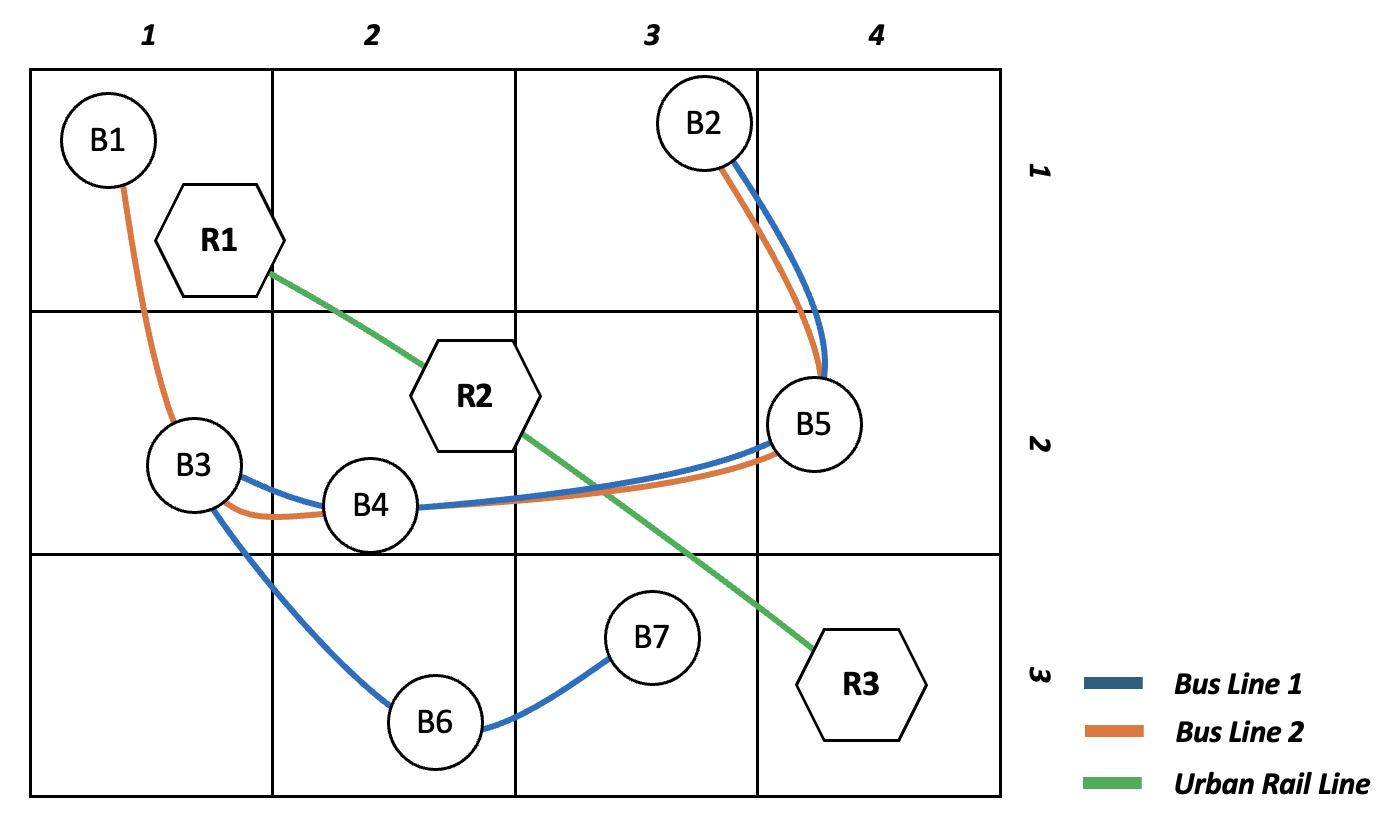
\includegraphics[width=.85\textwidth]{Figure/caseStudy.jpg}
\caption{Case Study Illustration} \label{fig:case_illustration}
\end{figure}
% ------------------------- FIGcaseEnd

To evaluate the effectiveness of the proposed framework under urban rail disruptions, we design a stylized case study on a small-scale synthetic network. The study area is constructed as a \(3 \times 4\) grid, where each tile centroid \(s \in \pazocal{S}\) represents a demand origin, and the public transport (PT) network consists of three urban rail stations supplemented by two bus lines. Within this grid, 99 opportunities are spatially distributed, thereby defining the spatial basis against which accessibility can be assessed. Building on this setup, accessibility is evaluated on the PT network by modeling tile centroids, stations, and opportunities as nodes, with edges encoding travel times as specified in Section~\ref{sec:TWA}. For each tile \(s\), the set of reachable opportunities \(\pazocal{O}_s\) is determined by computing shortest paths to all opportunities with Dijkstra’s algorithm under a 30-minute travel-time budget. In the baseline scenario, where no disruption is assumed, the nominal number of accessible opportunities \(|\pazocal{O}_s|\) from each tile is recorded. The overall setup is illustrated in Figure~\ref{fig:case_illustration}, and the corresponding parameters are summarized in Table~\ref{tab:case_parameters}.

As a preliminary experiment, we restrict our attention to \textbf{urban rail disruptions} and do not account for uncertainties in traffic variations. As a result, we exclude the effect of dedicated bus lanes, which are typically introduced to mitigate congestion. In our formulation, this is equivalent to setting $b_{ij} = 0$.
%
We then consider four urban rail disruption scenarios with probabilities 
\(\{0.5,\,0.2,\,0.2,\,0.1\}\): 
(i) no disruption, (ii) only R1--R2 disrupted, (iii) only R2--R3 disrupted, and (iv) both links disrupted. 
%
Given a disruption scenario, the PT network may evolve into different states depending on the operator’s response:
\begin{itemize}
    \item \emph{Nominal Baseline} (\(\pazocal G^O\)): the intact PT network under scenario (i) with no disruptions. 
    \item \emph{Unmitigated Disruption} (\(\pazocal G^\text{DISR}_\omega\)): the network resulting from scenario \(\omega\in\{ii,iii,iv\}\) when rail segments affected by the disruption are simply disabled and no remediation is applied. 
    \item \emph{Conventional Replacement Bus} (\(\pazocal G^\text{REPL}_\omega\)): the network under scenario \(\omega\) with additional buses operating along the disrupted urban rail link. This is the approach classically taken. However, it is important to consider that the speed of the replacement bus is generally much lower than the replaced rail since the bus has to travel on a road network, characterized by lower speed and higher circuitry.
    \item \emph{Our Solution} (\(\pazocal G^\text{OURS}_\omega\)): the optimized network produced by our stochastic programming model introduced in Section~\ref{sec:model} under scenario \(\omega\).
\end{itemize}

% --------------------------------- 5.2
\subsection{Performance of Our Solution}

We employ two scenarios--average indicators to evaluate the performance of different interventions. The first is the \emph{WA gain}, which measures the relative improvement of accessibility
compared with the disrupted network. It is defined as
\begin{equation}
\overline{\Delta}^\text{gain}_{\text{WA}}(\omega;\pazocal G^\ast)
= \frac{1}{|\pazocal S|}\sum_{s\in\pazocal S}
  \frac{A_{s}(\pazocal G^\ast_\omega) -
        A_{s}(\pazocal G^\text{DISR}_\omega)}
       {A_{s}(\pazocal G^\text{DISR}_\omega)},
\end{equation}
where $A_{s}(\cdot)$ denotes the accessibility of tile~$s$ under scenario~$\omega$. Positive values indicate that the intervention restores accessibility beyond the disrupted baseline.

The second indicator is the \emph{opportunity change}, which captures the variation in the number of opportunities reachable within the 30-minute threshold $\tau$:
\begin{equation}
\overline{\Delta}^{\text{opp}}(\omega;\pazocal G^\ast)
= \frac{1}{|\pazocal S|}\sum_{s\in\pazocal S}
  \Big(N^{30}_{s,\omega}(\pazocal G^\ast) -
       N^{30}_{s,\omega}(\pazocal G^\text{DISR})\Big),
\end{equation}
where $N^{30}_{s,\omega}(\pazocal G)$ denotes the number of opportunities in tile~$s$ that are reachable within 30 minutes under scenario~$\omega$. Negative values indicate a reduction in strict 30-minute reachability, while positive values imply that more opportunities become accessible.

Table~\ref{tab:wa_scenarios} reports the results for both indicators. Across all disruption scenarios, both the replacement bus and the optimized design substantially improve accessibility.
Nevertheless, the optimized design consistently achieves greater recovery, underscoring its superior ability to restore accessibility. In terms of 30-minute reachability, both strategies incur average
losses, confirming that the strict time threshold remains a binding constraint. 
%
However, the optimized design reduces these losses significantly relative to the replacement bus. 
%
Taken together, these results highlight the clear advantage of our method: by reallocating services toward time-critical origin--destination pairs, it delivers higher weighted accessibility while limiting the sacrifice of longer-distance opportunities.

\begin{table}[h]
\caption{Comparison of scenario--average performance: WA gains and 30-minute opportunity changes for the replacement bus and the optimized design.}
\label{tab:wa_scenarios}
\begin{tabular*}{\hsize}{@{\extracolsep{\fill}}lcccc@{}}
\toprule
Scenario & \multicolumn{2}{c}{WA Gain (tile avg.)} & \multicolumn{2}{c}{Opp.\ Change (tile avg.)}\\
\cmidrule(lr){2-3}\cmidrule(lr){4-5}
& Replacement Bus & Our Method & Replacement Bus & Our Method \\
\colrule
R1--R2 disrupted          & +11.92 & +12.15 & -2.2 & --0.6 \\
R2--R3 disrupted          & +11.30 & +12.13 & -2.3 & --0.3 \\
Both links disrupted      & +11.89 & +13.02 & -3.0 & --1.3 \\
\botrule
\end{tabular*}
\end{table}

% 2). 哪些候选站点被建设 (z_i)，dedicated lanes (b_ij) 的数量与位置
% 3). 保持原线路结构” 权衡。
% --- Intro text before the table ---
% 2). Infrastructure decisions (candidate stops, dedicated lanes) 
%     and line structure preservation

Since dedicated lanes are excluded in this setting ($b_{ij}=0$), we now examine the \textbf{proactive planning decisions}, namely the infrastructure measures that are made in advance of disruptions. In this context, the key choices concern which candidate stops to open and the extent to which the optimized bus network preserves the original line structure. Structural similarity is measured using the \emph{Path Overlap Retention Percentage (PORP)} introduced in Section~\ref{subsec:porp}.

\begin{table}[h]
\caption{Infrastructure decisions and line–structure preservation under
different disruption scenarios (without dedicated lanes).}
\label{tab:infra_decisions}
\begin{tabular*}{\hsize}{@{\extracolsep{\fill}}lcc@{}}
\toprule
Scenario & Selected Candidate Stops ($z_i$) & PORP \\ 
\colrule
R1--R2 disrupted     & C1, C3, C4 & 1.000 \\
R2--R3 disrupted     & C1, C3     & 0.667 \\
Both links disrupted & C1, C3, C4 & 0.875 \\
\botrule
\end{tabular*}
\end{table}

Across scenarios, the model selects a small subset of stops (typically two or three out of four), while preserving much of the original line structure. For example, when the R1--R2 link is disrupted, opening three stops achieves a \textbf{PORP of 1.000}, meaning the line order is fully retained. By contrast, the R2--R3 disruption produces the most adjustment, with only two stops selected and a lower \textbf{PORP of 0.667}. Overall, the results show that even with minimal infrastructure changes, the optimized design maintains high structural continuity, balancing adaptability with passenger familiarity.

% ------------------------------------------------------------
% 目前没有建立dedicateed lanes -》 因为没有考虑travel time的变化，后续会考虑
% ------------------------------------------------------------

% =============================================
% 6. Conclusion
% =============================================
\section{Conclusion and Future Work}
% 我们需要测试极端场景，即如果第一阶段过于鲁棒也许并不需要第二阶段？
This paper presented a proactive and adaptive optimization framework for improving the resilience of public transport systems during urban rail disruptions. On a stylized case study built on a synthetic grid network, the proposed method consistently outperformed conventional bus-bridging strategies: it delivered larger gains in time-weighted passenger accessibility and better preserved 30-minute reachability, yielding recovery outcomes that are both more effective and more equitable. The analysis also showed that preparing only a small set of candidate bus stops in advance can produce substantial benefits without materially altering the original line structure. Taken together, these results underscore the value of jointly optimizing accessibility restoration and operational continuity when managing disruptions.

While encouraging, the present study is best regarded as a proof of concept, and two directions stand out for future work. First, the framework should be applied to large-scale, real-world networks in order to assess its computational scalability and its practical performance under realistic operating conditions. Second, the current model does not fully capture the traffic dynamics induced by disrupted travel patterns, where reallocated demand can trigger congestion spillovers onto surrounding roads. Incorporating such network effects, for example through dedicated bus lanes or other congestion-mitigation measures, is a natural next step.

\section*{Acknowledgements}

This work has been supported by the French ANR research project MuTAS (ANR-21-CE22-0025-01).\\
We are grateful to the Gurobi Academic Program for providing Gurobi Optimizer, which was essential for our research.

%% The Appendices part is started with the command \appendix;
%% appendix sections are then done as normal sections
%% \appendix

%% \section{}
%% \label{}

% \appendix
% \section{An example appendix}
% Authors including an appendix section should do so before References section. Multiple appendices should all have headings in the style used above. They will automatically be ordered A, B, C etc.

% \subsection{Example of a sub-heading within an appendix}
% There is also the option to include a subheading within the Appendix if you wish.
% %% References
% %%
% %% Following citation commands can be used in the body text:
% %% Usage of \cite is as follows:
% %%   \cite{key}         ==>>  [#]
% %%   \cite[chap. 2]{key} ==>> [#, chap. 2]
% %%

% %The citation must be used in following style: \cite{article-minimal} \cite{article-full} \cite{article-crossref} \cite{whole-journal}.
% %% References with BibTeX database:

\bibliography{xampl}
\bibliographystyle{elsarticle-harv}


%% Authors are advised to use a BibTeX database file for their reference list.
%% The provided style file elsarticle-num.bst formats references in the required Procedia style

%% For references without a BibTeX database:

\clearpage

%%%% This page is for instructions only, once the article is finalize please omit the below text before creating the final PDF
\normalMode

\end{document}

%%
%% End of file.
